%%%%%%%%%%%%%%%%%%%%%%%%%%%%%%%%%%%%%%%%%%%%%%%%%%%%%%%%%%%
%% Principios del diseño

\section{Visión general del desarrollo y principios del diseño técnico}\label{principios:vision-general-desarrollo}

\subsection{Principios de diseño}\label{principios:principios-de-diseno}
Se pretende generar un código sólido, flexible y eficiente, pero el énfasis en esta primera etapa de desarrollo será hacia la \emph{flexibilidad}. En principio, la idea original de diseño es solo eso, una idea; a medida que se vaya obteniendo más información y \emph{aprendamos más del proceso de desarrollo y los requerimientos del diseño}, deberemos ir refactorizando el código\footnote{Reestructurar su estructura interna sin alterar su comportamiento externo.} para obtener unidades más definidas, mejor alineadas a los requerimientos y particularmente, que sean unidades fáciles de mantener.

Para ello, se deberá implementar un sistema de pruebas por cada feature que se trabaje. Esto implica invertir el proceso de desarrollo escribiendo primero el test, dejar que falle y a continuación implementar la funcionalidad. El principio es concentrarse en las pruebas no en el \foreignlanguage{english}{debugging}; aunque es ineludible, \emph{no queremos estar arreglando bugs, sino que queremos evitarlos}.

Se simplifica el diseño para agilizar el desarrollo y facilitar el mantenimiento.

\subsection{Desarrollo dirigido por tests (TDD)}\label{principios:TDD}
\subsection*{El qué antes del cómo}

\begin{figure}[ht]
	\centering
	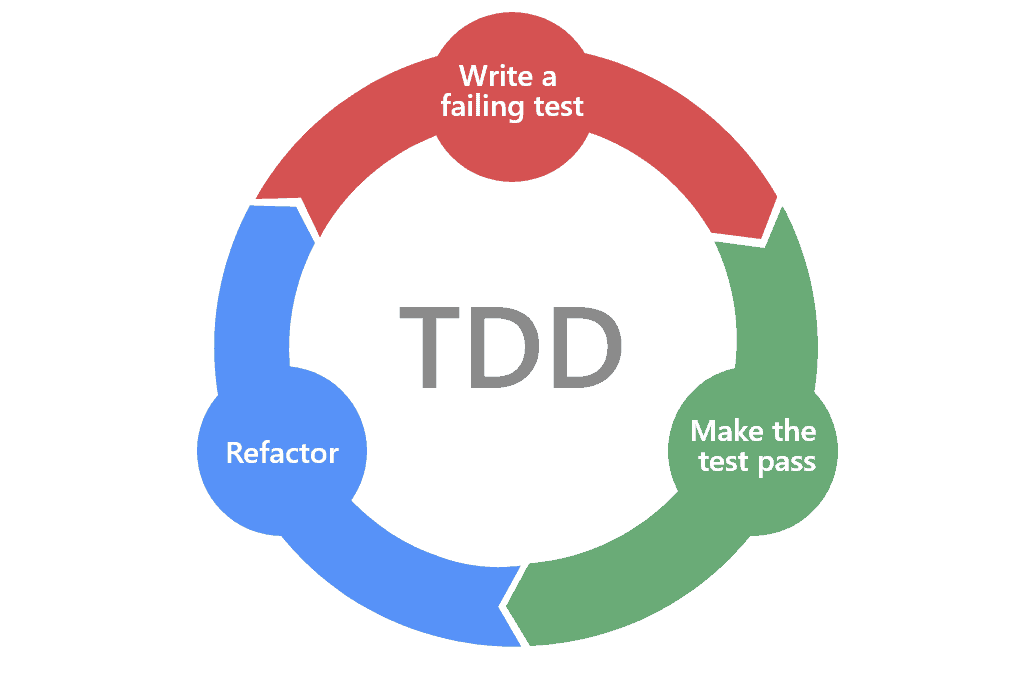
\includegraphics[width=0.75\textwidth]{imágenes/tdd.png}
	\caption{Flujo de desarrollo TDD.}
\end{figure}

Se comienza a trabajar por la fase roja escribiendo un test que supervise la implementación de la nueva funcionalidad. \emph{No queremos probar cómo funciona el código, sino probar que se comporte de la forma que esperamos}. Dado que aún el código no ha sido implementado este test fallará. Es importante no saltarse este paso y dejar que el test falle.

A continuación en la fase verde, se trabaja en la implementación del código tratando de superar el test de la forma más directa y rápida posible; \textit{no importa que el código sea horrible}.

Habiendo superado el test sabemos que contamos con un código que funciona, pasamos entonces a la fase azul donde refactorizamos este código ahora en búsqueda de eficiencia y limpieza. Ya que contamos con nuestros test unitarios, podremos saber en todo momento cuando nuestra refactorización es correcta o genera problemas.

Repetimos el ciclo hasta alcanzar nuestras metas de implementación.

Siguiendo esta metodología, se otorgará mayor flexibilidad para el diseño creativo del juego. Al mismo tiempo, dada la magnitud y complejidad de todo el sistema, ya que el testeo del código es parte del proceso de desarrollo, se pretende minimizar considerablemente la cantidad de bugs que llegue a la rama \textbf{main} (ver el apartado \nameref{flujo:repositorio}).

\subsection{Refactorización: Rendimiento y limpieza}\label{principios:refactorizacion-rendimiento-limpieza}
Aunque es frecuente limpiar el código a medida que se escribe, al hacer eso no estamos refactorizando; el factor clave de la refactorización es hacerlo intencionalmente pero de forma separada a la adición de nueva funcionalidad. \emph{Al ya tener definidas las pruebas, la reescritura del código se puede hacer con seguridad y confianza}.

El objetivo en este proceso es doble, por un lado se busca un rendimiento óptimo en los apartados que lo requieran (combate, IA, físicas y animación por ejemplo) y por otro la revisión del código además de mejorar la legibilidad del mismo (mejores nombres de funciones, variables y comentarios), nos ayuda al entendimiento del sistema y puede señalar oportunidades de encapsulación y mejoras al modelamiento.

\subsection{El documento de diseño técnico: una herramienta de diseño}\label{principios:documento-tecnico-como-herramienta}
El presente documento ha sido concebido como una potente herramienta de diseño, pues ofrece la oportunidad de reunir la gran cantidad de elementos relevantes para la construcción de este software en un solo lugar y por lo mismo, ordenar y sistematizar el proceso de producción en una manera coherente al proyecto y sus requerimientos.

Dado que Bakumapu se encuentra en estado de planificación o preproducción, el contar con un instrumento que reuna todas las dimensiones relevantes al desarrollo en un solo lugar, hace de su redacción y lectura un ejercicio de diseño. La continua revisión del texto servirá como una oportunidad para optimización y mejora en el software y en la adminsitración de los flujos de trabajo.

Los detalles con respecto al uso del texto se verán en detalle dentro del apartado \nameref{flujo:documento-de-diseno}.

Aplicando simplicidad junto al desarrollo colectivo de la documentación y el software, nos aseguramos que a medida que el código crezca, el equipo conocerá de manera más profunda y con mayor amplitud el sistema completo y la naturaleza de sus interacciones.
